% Created by tikzDevice version 0.12.3.1 on 2022-09-02 13:46:12
% !TEX encoding = UTF-8 Unicode
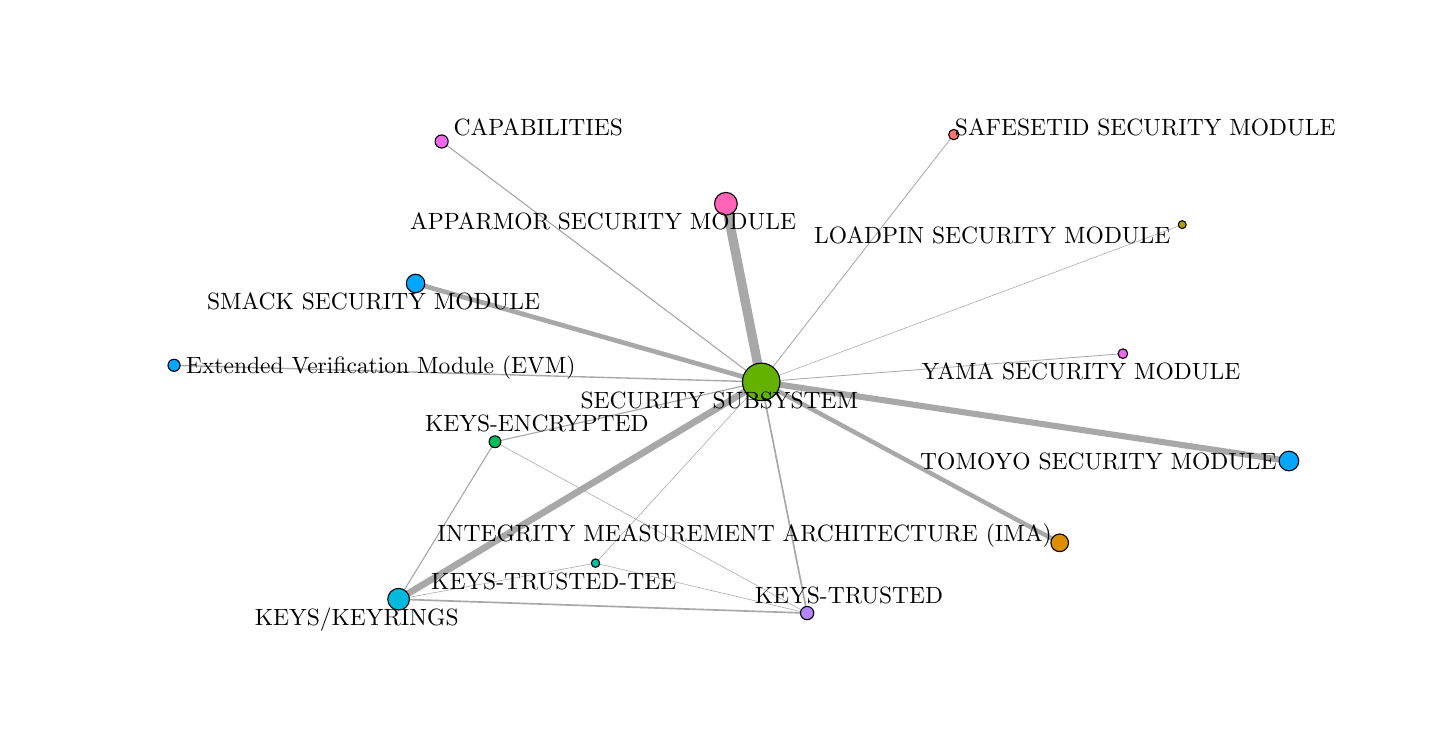
\begin{tikzpicture}[x=1pt,y=1pt]
\definecolor{fillColor}{RGB}{255,255,255}
\path[use as bounding box,fill=fillColor,fill opacity=0.00] (0,0) rectangle (505.89,252.94);
\begin{scope}
\path[clip] (  0.00,  0.00) rectangle (505.89,252.94);
\definecolor{fillColor}{RGB}{255,255,255}

\path[fill=fillColor] (  0.00,  0.00) rectangle (505.89,252.94);
\end{scope}
\begin{scope}
\path[clip] ( 32.75, 32.75) rectangle (475.89,222.94);
\definecolor{drawColor}{gray}{0.66}

\path[draw=drawColor,line width= 3.4pt,line join=round] (252.30,189.30) -- (265.07,124.94);

\path[draw=drawColor,line width= 0.4pt,line join=round] (149.58,211.81) -- (265.07,124.94);

\path[draw=drawColor,line width= 0.5pt,line join=round] ( 52.89,130.93) -- (265.07,124.94);

\path[draw=drawColor,line width= 1.6pt,line join=round] (372.92, 66.79) -- (265.07,124.94);

\path[draw=drawColor,line width= 0.2pt,line join=round] (168.86,103.31) -- (281.65, 41.40);

\path[draw=drawColor,line width= 0.4pt,line join=round] (168.86,103.31) -- (134.04, 46.41);

\path[draw=drawColor,line width= 0.4pt,line join=round] (168.86,103.31) -- (265.07,124.94);

\path[draw=drawColor,line width= 0.2pt,line join=round] (281.65, 41.40) -- (205.19, 59.44);

\path[draw=drawColor,line width= 0.6pt,line join=round] (281.65, 41.40) -- (134.04, 46.41);

\path[draw=drawColor,line width= 0.6pt,line join=round] (281.65, 41.40) -- (265.07,124.94);

\path[draw=drawColor,line width= 0.2pt,line join=round] (205.19, 59.44) -- (134.04, 46.41);

\path[draw=drawColor,line width= 0.2pt,line join=round] (205.19, 59.44) -- (265.07,124.94);

\path[draw=drawColor,line width= 2.4pt,line join=round] (134.04, 46.41) -- (265.07,124.94);

\path[draw=drawColor,line width= 0.2pt,line join=round] (417.19,181.76) -- (265.07,124.94);

\path[draw=drawColor,line width= 0.3pt,line join=round] (334.65,214.30) -- (265.07,124.94);

\path[draw=drawColor,line width= 1.7pt,line join=round] (265.07,124.94) -- (140.16,160.50);

\path[draw=drawColor,line width= 2.2pt,line join=round] (265.07,124.94) -- (455.75, 96.35);

\path[draw=drawColor,line width= 0.3pt,line join=round] (265.07,124.94) -- (395.76,135.14);
\definecolor{drawColor}{RGB}{0,0,0}
\definecolor{fillColor}{RGB}{255,99,182}

\path[draw=drawColor,line width= 0.4pt,line join=round,line cap=round,fill=fillColor] (252.30,189.30) circle (  4.11);
\definecolor{fillColor}{RGB}{239,103,235}

\path[draw=drawColor,line width= 0.4pt,line join=round,line cap=round,fill=fillColor] (149.58,211.81) circle (  2.37);
\definecolor{fillColor}{RGB}{0,166,255}

\path[draw=drawColor,line width= 0.4pt,line join=round,line cap=round,fill=fillColor] ( 52.89,130.93) circle (  2.18);
\definecolor{fillColor}{RGB}{219,142,0}

\path[draw=drawColor,line width= 0.4pt,line join=round,line cap=round,fill=fillColor] (372.92, 66.79) circle (  3.19);
\definecolor{fillColor}{RGB}{0,189,92}

\path[draw=drawColor,line width= 0.4pt,line join=round,line cap=round,fill=fillColor] (168.86,103.31) circle (  2.13);
\definecolor{fillColor}{RGB}{179,133,255}

\path[draw=drawColor,line width= 0.4pt,line join=round,line cap=round,fill=fillColor] (281.65, 41.40) circle (  2.40);
\definecolor{fillColor}{RGB}{0,193,167}

\path[draw=drawColor,line width= 0.4pt,line join=round,line cap=round,fill=fillColor] (205.19, 59.44) circle (  1.52);
\definecolor{fillColor}{RGB}{0,186,222}

\path[draw=drawColor,line width= 0.4pt,line join=round,line cap=round,fill=fillColor] (134.04, 46.41) circle (  3.92);
\definecolor{fillColor}{RGB}{174,162,0}

\path[draw=drawColor,line width= 0.4pt,line join=round,line cap=round,fill=fillColor] (417.19,181.76) circle (  1.43);
\definecolor{fillColor}{RGB}{248,118,109}

\path[draw=drawColor,line width= 0.4pt,line join=round,line cap=round,fill=fillColor] (334.65,214.30) circle (  1.86);
\definecolor{fillColor}{RGB}{100,178,0}

\path[draw=drawColor,line width= 0.4pt,line join=round,line cap=round,fill=fillColor] (265.07,124.94) circle (  6.78);
\definecolor{fillColor}{RGB}{0,166,255}

\path[draw=drawColor,line width= 0.4pt,line join=round,line cap=round,fill=fillColor] (140.16,160.50) circle (  3.34);

\path[draw=drawColor,line width= 0.4pt,line join=round,line cap=round,fill=fillColor] (455.75, 96.35) circle (  3.55);
\definecolor{fillColor}{RGB}{239,103,235}

\path[draw=drawColor,line width= 0.4pt,line join=round,line cap=round,fill=fillColor] (395.76,135.14) circle (  1.74);

\node[text=drawColor,anchor=base,inner sep=0pt, outer sep=0pt, scale=  0.85] at (207.94,179.88) {APPARMOR SECURITY MODULE};

\node[text=drawColor,anchor=base,inner sep=0pt, outer sep=0pt, scale=  0.85] at (184.53,214.05) {CAPABILITIES};

\node[text=drawColor,anchor=base,inner sep=0pt, outer sep=0pt, scale=  0.85] at (127.60,127.99) {Extended Verification Module (EVM)};

\node[text=drawColor,anchor=base,inner sep=0pt, outer sep=0pt, scale=  0.85] at (259.08, 67.11) {INTEGRITY MEASUREMENT ARCHITECTURE (IMA)};

\node[text=drawColor,anchor=base,inner sep=0pt, outer sep=0pt, scale=  0.85] at (183.97,106.87) {KEYS-ENCRYPTED};

\node[text=drawColor,anchor=base,inner sep=0pt, outer sep=0pt, scale=  0.85] at (296.80, 44.95) {KEYS-TRUSTED};

\node[text=drawColor,anchor=base,inner sep=0pt, outer sep=0pt, scale=  0.85] at (190.10, 50.02) {KEYS-TRUSTED-TEE};

\node[text=drawColor,anchor=base,inner sep=0pt, outer sep=0pt, scale=  0.85] at (118.91, 36.99) {KEYS/KEYRINGS};

\node[text=drawColor,anchor=base,inner sep=0pt, outer sep=0pt, scale=  0.85] at (348.56,175.12) {LOADPIN SECURITY MODULE};

\node[text=drawColor,anchor=base,inner sep=0pt, outer sep=0pt, scale=  0.85] at (403.84,214.05) {SAFESETID SECURITY MODULE};

\node[text=drawColor,anchor=base,inner sep=0pt, outer sep=0pt, scale=  0.85] at (249.96,115.50) {SECURITY SUBSYSTEM};

\node[text=drawColor,anchor=base,inner sep=0pt, outer sep=0pt, scale=  0.85] at (124.99,151.07) {SMACK SECURITY MODULE};

\node[text=drawColor,anchor=base,inner sep=0pt, outer sep=0pt, scale=  0.85] at (386.93, 93.41) {TOMOYO SECURITY MODULE};

\node[text=drawColor,anchor=base,inner sep=0pt, outer sep=0pt, scale=  0.85] at (380.62,125.69) {YAMA SECURITY MODULE};
\end{scope}
\end{tikzpicture}
